\documentclass[]{article}
\usepackage[round]{natbib}
\usepackage{geometry}               % See geometry.pdf to learn layout options
\geometry{letterpaper}              % ... or a4paper or a5paper or ... 
%\usepackage[parfill]{parskip}      % Activate to begin paragraphs with an
                                    %   empty line rather than an indent
\usepackage{graphicx}               % Use pdf, png, jpg, or eps with pdflatex;
                                    %   use eps in DVI mode;
                                    %   TeX automatically converts
                                    %     eps --> pdf in pdflatex                
\usepackage{amsmath}
\usepackage{amssymb}
\usepackage{upquote}

%-----------------------------------------------------------------------------
% Special-purpose color definitions (dark enough to print OK in black and white)
\usepackage{color}
% A few colors to replace the defaults for certain link types
\definecolor{orange}{cmyk}{0,0.4,0.8,0.2}
\definecolor{darkorange}{rgb}{.71,0.21,0.01}
\definecolor{darkgreen}{rgb}{.12,.54,.11}
%-----------------------------------------------------------------------------
% The hyperref package gives us a pdf with properly built
% internal navigation ('pdf bookmarks' for the table of contents,
% internal cross-reference links, web links for URLs, etc.)
\usepackage{hyperref}
\hypersetup{pdftex, % needed for pdflatex
  breaklinks=true, % so long urls are correctly broken across lines
  colorlinks=true,
  urlcolor=blue,
  linkcolor=darkorange,
  citecolor=darkgreen,
}

%-----------------------------------------------------------------------------
%
% Commands for annotating the docs with fixme and inter-author notes.  See
% below for how to disable these.
%
% Define a \fixme command to mark visually things needing fixing in the draft,
% as well as similar commands for each author to leave initialed special
% comments in the document.
% For final printing or to simply disable these bright warnings
% by uncommenting lines below "to turn all the special marker commands off"

\newcommand{\fix}[1] { \textcolor{red} {
{\fbox{ {\bf Fix:} \ensuremath{\blacktriangleright }} {\bf #1}
\fbox{\ensuremath{\blacktriangleleft} } } } }

% And similarly, one (less jarring, with fewer symbols and no boldface) command
% for each one of us to leave comments in the main text.
\newcommand{\philip}[1] { \textcolor{blue} {
\ensuremath{\blacklozenge} {\bf philip:}  {#1}
\ensuremath{\blacklozenge} } }

\newcommand{\jarrod}[1] { \textcolor{darkgreen} {
\ensuremath{\bigstar} {\bf jarrod:}  {#1}
\ensuremath{\bigstar} } }

\newcommand{\kellie}[1] { \textcolor{darkorange} {
\ensuremath{\blacksquare} {\bf kellie:}  {#1}
\ensuremath{\blacksquare} } }

%% Uncomment these to turn all the special marker commands off
%\renewcommand{\fix}[1]{}
%\renewcommand{\philip}[1]{}
%\renewcommand{\jarrod}[1]{}
%\renewcommand{\kellie}[1]{}


\date{}

\begin{document}

\title{A case study in reproducible applied statistics:\\
Is tagging of therapist-patient interactions reliable?
}

\author{K. Jarrod Millman (JM)\\ Division of Biostatistics\\ UC Berkeley \and
Kellie Ottoboni (KO)\\ Department of Statistics\\ UC Berkeley \and
Naomi A. P. Stark (NS)\\ Department of Philosophy\\ University of Pennsylvania \and
Philip B. Stark (PS)\\ Department of Statistics\\ UC Berkeley
}

\maketitle


\section{Introduction}

This case study\footnote{This file along, with the analysis script and results,
can be found here: \url{https://github.com/statlab/nsgk}}.
That repository illustrates some of
the reproducible practices we (JM, KO, PS) have adopted.
Parts of the text have been adapted from \citet{millman2015thesis} and a
shorter version was submitted to
\url{https://github.com/BIDS/repro-case-studies}.


\begin{enumerate}
\def\labelenumi{\arabic{enumi})}
\itemsep1pt\parskip0pt\parsep0pt
\item
  Who are you and what is your research field?
\end{enumerate}

We are three applied statisticians~(JM,~KO,~PS) at U.C. Berkeley working with a
domain specialist~(NS) at the University of Pennsylvania.
Our case study involves assessing inter-rater reliability (IRR) for human
classifiers of behavior during therapy sessions with children on the autistic spectrum.

\begin{enumerate}
\def\labelenumi{\arabic{enumi})}
\setcounter{enumi}{1}
\itemsep1pt\parskip0pt\parsep0pt
\item
  Define what the term ``reproducibility'' means to you generally and/or
  in the particular context of your case study.
\end{enumerate}

In this case study, \emph{reproducibility} means that we have documented 
(and scripted) nearly
every step of the analysis---from cleaning to coding to code execution---as
well as much of the discussion preceding our decision to take those steps.
It also means that we have tested our code thoroughly and in an automated fashion, 
to have justifiable confidence that the code does what it was intended
to do.
Finally, it also means that we invested time to understand the fundamental
problem and the results of our analysis so that we do \emph{not} make
conclusions that are not justified by the data, the manner in which it was
acquired, and our domain understanding.

By keeping all code, text, and data in a public version-controlled repository, 
we have made our well-documented analysis available
for anyone to examine, check, modify, or re-use.
We have released the data used in our study---both the original anonymized
version as well as our cleaned version including the commands necessary
to produce the cleaned version from the anonymized one.
In addition to making what we did transparent to anyone who is interested,
working in this way means that when errors are found we can identify
how and when those errors were introduced.
We have written tests for almost all our code, which means we have a high
level of confidence that as we change our code we will catch any errors
we might have introduced, and can correct them quickly and easily.
And since we have automated the process of running our analysis, if errors
are identified and corrected, it is easy to rerun the entire analysis from
start to finish.

If you have standard tools (see \S~\ref{key-tools}) installed on your
computer and network access, you can run our complete analysis of the cleaned
data by typing the following three commands from a unix shell prompt:
\begin{verbatim}
$ git clone git@github.com:statlab/nsgk.git
$ cd nsgk/nsgk
$ make
\end{verbatim}
The first command creates a directory \texttt{nsgk} in your current working
directory with a copy of the project repository (i.e., a directory with our
code, data, and text along with the provenance of these documents).
This directory contains this document as well as everything needed to run our
analysis.
Inside \texttt{nsgk/nsgk} there is a \texttt{Makefile}, our analysis script
\texttt{analysis.py}, and the output \texttt{results.csv} of that script.

When you enter the command \texttt{make}, the following commands will be run:
\begin{verbatim}
virtualenv -p /usr/bin/python2.7 venv
venv/bin/pip install --upgrade pip
venv/bin/pip install -r requirements.txt
venv/bin/python analysis.py
\end{verbatim}
The first command creates a new virtual environment (\texttt{venv}) for Python~2.7.
Using this new virtual environment (\texttt{venv}) the subsequent commands
respectively upgrade the Python package manager (\texttt{pip}) to the most
recent version, install the necessary Python package dependencies
(\texttt{numpy~1.11.0}, \texttt{scipy~0.17.0}, and \texttt{permute~0.1a2}),
and run the analysis script \texttt{analysis.py}.

\section{Workflow narrative}\label{workflow-narrative}

Our project arose from a pilot study NS was working on with Dr.~Gilbert Kliman of
the Children's Psychological Health Center in San Francisco.
To investigate therapeutic interventions in children on the autism scale,
Dr. Kliman and NS collected some observational data (described below).
NS approached PS about her data and
the problem NS was interested in addressing.
After investigating the problem further, PS emailed JM and KO a one-page
proposal for a stratified permutation test to assess inter-rater
reliability using stratified samples.
We (JM, KO, PS) had recently begun developing a general purpose Python package
for permutation tests, called
\texttt{permute}\footnote{\url{http://statlab.github.io/permute/}},
based on our collaborations.
PS suggested this would be an interesting example to include.

After coming to an initial understanding of NS's underlying research question
and experiment, including how her data were collected, we (JM, KO, PS) 
cleaned the data, developed a nonparametric approach to assessing IRR
appropriate to the experiment, implemented the approach in Python, incorporated
the resulting code into our evolving Python package of permutation tests,
applied the approach to the cleaned data, documented the code and the analysis,
and wrote up the results in \LaTeX. 

We distinguish the following aspects of our project, which are typical in
applied statistics:
\begin{itemize}
    \item understand problem
    \item get and clean data\footnote{
        This step generally also requires obtaining a data dictionary, learning
        how to parse the data format, and so on.
        }
    \item design algorithm
    \item implement algorithm
    \item analyze data
    \item understand result
\end{itemize}
Figure~\ref{fig:work_process} shows how each aspect of the
project influenced the other aspects and gives estimates of the total person-hours
we collectively spent on each aspect of the project.
For example, if all three of us (JM, KO, PS) spent an hour discussing the
problem in a meeting, then that hour involved 3 people hours.
\jarrod{Need to explain why we are using names and time estimates since
we were asked to remove them.
- give people an idea how ``inexpensive'' (or expensive) working more
  reproducibly is.
- capture how group understanding evolved
- hope that it might be instructive for students and collaborators
}

\begin{figure}[h]
  \centering
    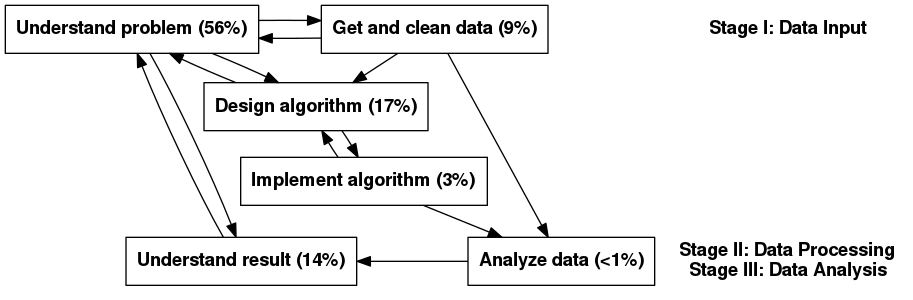
\includegraphics[width=0.8\textwidth]{_fig/work_process_bids.png}
  \caption{
  \small
    Each box corresponds to one aspect of the project.
    The percents are estimates of the percent of our time spent on each aspect.
    Edges represent influence.
    \texttt{Understand problem}~$\to$~\texttt{Design algorithm}, for instance,
    corresponds to the fact that we had to understand the problem in order to
    design the correct statistical test.\label{fig:work_process}}
\end{figure}

Since we view computational reproducibility as a cross-cutting concern of all
project aspects, we have adopted a set of computational practices, which we
(JM, KO, PS) followed (almost) whenever we were working on the
project.\footnote{Exceptions include that we did not record all of our
in-person discussions or whiteboard work.  
However, we endeavored to
record summaries of these activities.}
These computational practices are described in \citet{millman2014developing}
and are used widely in the open source scientific Python community.
While developed for managing software contributions, these practices are ideal
for ensuring computational reproducibility in scientific and statistical
research.
We will illustrate how we leverage the software infrastructure and development
practices of \texttt{permute} to conduct reproducible and collaborative applied
statistics research with our colleagues.
We discuss the software tools and practices briefly in \S~\ref{key-tools} below.

\subsection{Understand problem (80 hours)}
The Kliman-Stark research project sought to identify characteristics of 
effective clinical interactions with children on the autistic spectrum.
The project first required developing a set of characteristics that observers
could use to ``tag'' what was happening in each 30-second interval of a 
therapy session.
After they developed a taxonomy of clinical interactions, Kliman and NS had a 
number of trained raters watch videos of therapy sessions and label each 
30-second interval using the collection of tags.
For the classification system to be meaningful and useful, different
raters must generally agree on whether a given tag applies to a given video segment:
there must be inter-rater reliability.
Of course, if a tag is never used or is always used, inter-rater reliability will be perfect,
but the tag is useless.

That led to a statistical question: how to assess the evidence in the tagged videos
that different raters
tag interactions the same way? 
After numerous conversations, it made sense to consider the null hypothesis to be
that, conditional on the number of times a given rater applied a given label to
a given video, all assignments of that label to time stamps in the video are equally
likely, and the ratings given by different raters are exchangeable (essentially, that
raters are independent).

Once PS had an initial understanding of NS's problem, we (JM, KO, PS) met
regularly (approximately weekly, sometimes more) as a team to discuss the
project.
Initially these discussions involved a lot of work on whiteboards and asking a
lot of probing and open-ended questions.
This helped us develop a shared understanding of the problem, understanding
that improved by explaining it to one
another and by asking hard questions about our planned approach and whether
it could address the question of interest.
As our understanding of the problem progressed, our work transitioned from
working on whiteboards to testing our ideas out on a computer.
We often used pair programming at this stage and sometimes we (JM, KO, PS)
all sat in front of one computer, while one of us typed code in an interactive
IPython session.
This helped ensure that we all understood the problem well and it also helped
us catch errors (typos as well as conceptual errors).
%Time: approximately 10 2-hour meetings.

\subsection{Get and clean data (13 hours)}

The tag data were collected by NS and raters working at her direction.
The data comprise ratings of segments of 8~videos by 10~trained raters.
Each video is divided into approximately 40~time segments.
In each time segment, none, any, or all of 183~types of activity might be
taking place.
The raters indicated which of those activities was taking place during each
segment of each video.

PS received the data from NS as an Excel spreadsheet that had been entered
by hand by NS and an assistant.
Understanding the ``data dictionary'' and vetting for obvious errors entailed
several rounds of email between PS and NS before PS had a version of the data
that did not have obvious errors.
%Time: approximately 5 hour
PS then exported the Excel data to comma-separated value (CSV) format.
%Time: approximately 5 minutes.
The original data contained personal identifying information.
Using regular expressions in an interactive text editor, PS substituted
unique numerical identifiers for raters' names in the CSV file.
While this step was not performed reproducibly (i.e., not scripted), it can be
checked readily.
%Time: approximately 1 hour.

After PS generated the original anonymized data, JM committed it to our
repository and added a data loader with tests to ensure that if the data
changed we would know.
At this point, we (JM, PS) screened the anonymized data for transcription
errors (e.g., duplicate rows).
This involved writing a number of quality assurance tools (e.g., to find
duplicate consecutive rows), which are now included in \texttt{permute}.
%Time: approximately 5 hours
Once we identified entries incompatible with our understanding of what should
be in the data, JM wrote a \texttt{sed} script to ``correct'' the inferred
typos.
%Time: included above
The exact commands used to clean the data are included in the commit
corresponding to that cleaning step.
After carefully examining the data for potential errors and documenting
every change we made and why, we sent the cleaned data and an explanation
of what we did to NS to verify that the corrections were appropriate.
%Time: 1 hour
As a result, we provide the cleaned data in our project repository as well
as a careful account of its provenance.

\subsection{Design algorithm (25 hours)}

Although we eventually implemented something close to the original test
proposed by PS at the start of the project, we (JM, KO, PS) spent significant
time focused on ``problem appreciation.''
We also developed a more general terminology (see Table \ref{table:mapping}).
\begin{table}[h]
\begin{center}
\begin{tabular}{ | c | c | }
  \hline
  \textbf{NSGK} & \textbf{IRR}  \\
  \hline
  183 types of activity  & $T$ tags  \\
  \hline
  8 videos  & $S$ strata   \\
  \hline
  ~40 segments/videos  & $N_s$ items/strata   \\
  \hline
  10 raters  & $R$ raters  \\
  \hline
\end{tabular}
\caption{Mapping between terms from our motivating problem (NSGK) and the terms
         used in our general algorithm (IRR).}\label{table:mapping}
\end{center}
\end{table}

We decided to assess rater reliability in identifying (i.e., tagging)
each of the 183 types of activity separately.
\philip{
This decision introduced a multiple comparison problem, which we discuss in
\S~\ref{subsec:understand-result}.
}
%Time: approximately 4h.
Since each of the videos contained different sessions of therapist-patient
interactions, we decided to stratify our test by video.
A literature search for approaches to assessing IRR led us to conclude that
there was no existing suitable method for several reasons:
because the experiment was stratified,
because there were multiple raters to compare,
and because standard methods make indefensible parametric
assumptions, which we hoped to avoid.
%Time: 3h

After deciding to use permutation tests, we (JM, KO, PS) then determined what
the appropriate permutation would be: permuting each rater's ratings within a
video, independently across raters and across videos.
We chose to use concordance of ratings as our partial test statistic within
each stratum.
We (JM, PS) derived a simple expression for efficiently computing the
concordance.
%Time: 1h
To combine tests across strata, we (JM, KO, PS) decided to use the nonparametric
combination (NPC) of tests \citep{pesarin2010permutation}.
%Time: 1h
Finally, we (JM, KO, PS) developed a computationally efficient approach to
finding the overall $p$-value for the NPC test.
%Time: 1.5h

\subsection{Implement algorithm (5 hours)}

Once we had a blueprint of the algorithm, KO started to implement it.
While KO did most of the coding, JM and PS reviewed and discussed the
implementation.
Following our software development practices (\S~\ref{key-tools}), KO also
wrote tests for every function she implemented.
After a few iterations of coding, testing, and review, KO finalized our implementation
and we merged it into \texttt{permute}.

KO wrote three functions to implement our general IRR algorithm:
\begin{enumerate}
\item a function to compute the IRR partial test statistic from a binary
  matrix with one row per rater and one column per item;
\item a function to simulate the permutation distribution of the IRR partial
  test statistic for a matrix of ratings of a single stratum;
\item a function to simulate the permutation distribution of the NPC
  test statistic by combining the $S$ distributions of the IRR partial test 
  statistic for each of the $S$ strata.
\end{enumerate}

\subsection{Analyze data (1 hour)}

Once we merged KO's implementation of the general algorithm (including tests)
into \texttt{permute}, KO wrote a short script (about 50 lines of Python) to
analyze the cleaned data from NS.

Since the main workhorse functions were contained in \texttt{permute}, 
the analysis script contained only high-level commands:
\begin{enumerate}
\item Load the cleaned data
\item For each of the 183 categories of activity:
  \begin{enumerate}
    \item For each of the 8 videos:
    \begin{enumerate}
      \item Compute the mean and standard deviation of times the
        tag was observed
      \item Compute the IRR partial test statistic
    \end{enumerate}
    \item Simulate the permutation distribution of the NPC test statistic for each
    category, combining over the $8$ videos, and report a single $p$-value
  \end{enumerate}
\item Save the results to a CSV file.
\end{enumerate}


\subsection{Understand result (20 hours)}\label{subsec:understand-result}

\philip{You will probably want to wait until I have written up the results to
work on this; but, eventually we need a discussion of our final thoughts about
the data and how it did or did not address the question.  Maybe a sentence or
two saying what we learned...what we do differently during data collection next
time.  Understanding result can lead to 1) designing new experiment, 2)
collecting new data, 3) performing different analysis, 4) writing manuscript,
5) something else.  Need to connect this back to the our understanding of the
problem.  We should also say that despite not pursuing this further, it did
yield a new permutation test that could be used in other contexts and which is
available in \texttt{permute}.  }

\philip{
maybe scientific vs statistical significance, multiple comparison, selective
inference, etc.
}

\section{Pain points}\label{pain-points}

Given our different backgrounds and experiences we (JM, KO, PS) each found
different points in the process challenging. 
However, for all of us the most challenging aspect---and the most 
time-consuming---was the necessary
struggle to understand the scientific question and the experiment
well enough to devise an approach to answering the question.

For KO and PS there was a learning curve to master the tools and practices.
This involved understanding the data model used by Git, acquiring habits such
as writing tests for all functions and following a common style guide, and
learning to contribute to the project repository indirectly through GitHub's
pull request mechanism.
JM was already familiar with the tools and practices, and devoted significant time
to teaching KO and PS the workflow.
Once mastered, the benefits of these tools and habits outweigh the time and effort
spent learning them.

For JM the most painful part of the project was vetting hand-entered data
to look for errors and inconsistencies.
Not only was this laborious, but it involved inferring what the data
should have been without any direct way to ensure that these inferences were
correct.
The solution to this pain point is to automate the data collection process as
much as possible.
However, when data have already been entered by hand, there is not much that can
be done other than being cautious when ``fixing'' data entry errors and recording
every aspect of the data cleaning process.

\section{Key benefits}\label{key-benefits}

Since \citet{buckheit1995wavelab} popularized the idea of computational
reproducibility, applied statisticians have increasingly embraced version control
and process automation.
Many of our colleagues have made the idea of computational reproducibility
central in both the classroom and the lab.
Some ask anyone working with them to follow a set of computational practices
including version control.\footnote{
  For example, see
  \url{http://www.stat.berkeley.edu/~epurdom/studentResources.html}.
}

However, the computational practices described in this study
(see \S~\ref{key-tools}) go beyond the standard work habits of our colleagues.
Our computational practices provide the following benefits:
(1) a reduction in the number of errors introduced by new code and changes to
    existing code;
(2) it is easy to modify the analysis when errors are found, to apply the
    analysis to new data sets, and so on;
(3) the process is self-documenting, making it easier to draft a paper about
    the results; and
(4) the methods are abstracted from the analysis and incorporated into a
    package so that others can discover, check, use, and extend our methods.

\section{Key tools and practices}\label{key-tools}

As part of the development of our software package \texttt{permute}, we
invested significant effort in setting up a development infrastructure to
ensure our work is tracked, thoroughly and continually tested, and
incrementally improved and documented.
To this end, we have adopted best practices for software development used by
successful open source projects \citep{millman2014developing}.

\subsection{\label{sec:vc}Version control and code review}

We (JM, KO, PS) use Git\footnote{\url{http://git-scm.com}} as our version
control system (VCS) and GitHub\footnote{\url{https://github.com}} as the
public hosting service for our official \texttt{upstream} repository
(\url{https://github.com/statlab/permute}).
Each of us has our own copy, or fork, of the \texttt{upstream} repository.
We each work on our own repositories and use the \texttt{upstream} repository
as our coordination or integration repository.

This allows us to track and manage how our code changes over time as well as
review all new functionality before merging it into the \texttt{upstream}
repository.
To get new code or text integrated in the \texttt{upstream} repository, we use
GitHub's \emph{pull request} mechanism.
This enables us to review code and text before integrating it.
Below, we describe how we automate testing our code to generate reports for all
pull requests.
This way we can reduce the risk that changes to our code break existing
functionality.
Once a pull request is reviewed and accepted, it is merged into the
\texttt{upstream} repository.

Requiring all new code to undergo review provides several benefits.
Code review increases the quality and consistency of our code.
It helps maintain a high level of test coverage (see below).
Moreover, it also helps keep the development team aware of the work other team
members are doing.
While we are currently a small team and we meet regularly, having the code
review system in place will make it easier for new people to contribute as well
as capturing our design discussions and decisions for future reference.

\subsection{\label{sec:test}Testing and continuous integration}

We use the \texttt{nose} testing framework for automating our testing
procedures.\footnote{\url{https://nose.readthedocs.org}}
This is the standard testing framework\footnote{
    As \texttt{nose} has been in
    maintenance mode for the last few years, projects are starting to look
    into newer testing frameworks.
    We are migrating to \texttt{pytest} (\url{http://pytest.org}).
    While we may transition to a new testing framework, any system we
    migrate to will have the same basic features and benefits as \texttt{nose}.
}
used by the core packages in the scientific Python ecosystem.
Automating the tests allows us to monitor a proxy for code correctness when
making changes as well as simplifying the code review process for new code.
Without automated testing, we would have to manually test all the code every
time a change is proposed.
The \texttt{nose} testing framework simplifies test creation, discovery, and
running.
It has an extensive set of plugins to add functionality for coverage reporting,
test annotation, profiling, as well as inspecting and testing documentation.

\begin{figure}
  \begin{centering}
    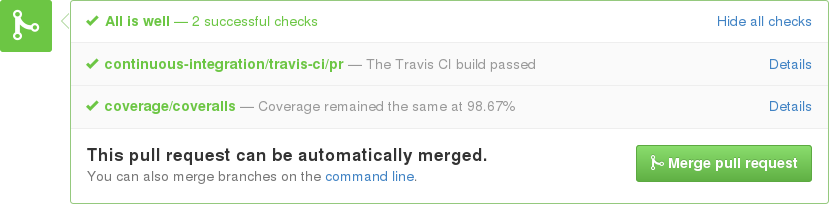
\includegraphics[width=\textwidth]{_fig/pull-request-ci.png}\par
  \end{centering}

  \caption{\label{fig:pull-request}
  \small
    Each pull request triggers an automated system to run the full test suite on
    the updated code.
    This means that when you go to review a pull request you can immediately see
    whether the change breaks any of the tests as well as whether the new
    code decreases the overall test coverage.
    For example, the above report indicates that the associated pull request does not
    break existing code and does not change our test coverage.}
\end{figure}

Our goal is to test every line of code.
For example, not only do we want to test every function in our package, but if
a specific function has internal logic we want to test each possible execution
path through the function.
Having tested each line of code increases our confidence in our code, but
more importantly provides us some measure of assurance that changes we make do
not break existing code.
It also increases our confidence that new code works, which reduces the
friction of accepting contributions.
Currently over 98\% of \texttt{permute}'s lines of code get executed at least
once by our test system.

We have configured Travis CI\footnote{
  \url{https://travis-ci.org}
} 
and
\texttt{coveralls}\footnote{
  \url{https://coveralls.io}
}
to be automatically
triggered whenever a commit is made to a pull request or the upstream master
(see Figure~\ref{fig:pull-request}).
These systems run the full test suite using different versions of our
dependencies (e.g., Python 2.7 and 3.4) every time a new commit is made to a
repository or pull request.
\jarrod{Explain Travis CI and coveralls}

\subsection{\label{sec:doc}Documentation}

We use Sphinx\footnote{
   \url{http://sphinx-doc.org}
} 
as our documentation system
and already have good developer documentation and the foundation for
high-quality user documentation.
Sphinx is the standard documentation system for Python projects and is used by
the core scientific Python packages.
We use Python docstrings and follow the NumPy docstring
standard\footnote{
   \url{https://github.com/numpy/numpy/blob/master/doc/HOWTO\_DOCUMENT.rst.txt}
}
to document all the modules and functions in \texttt{permute}.
Using Sphinx and some NumPy extensions, we have a system for autogenerating the
project documentation (as HTML or PDF) using the docstrings as well as
stand-alone text written in a light-weight markdown-like language, called
reStructuredText\footnote{\url{http://docutils.sourceforge.net/rst.html}}.
This system enables us to easily embed references, figures, code that is
auto-run during documentation generation, as well as mathematics using \LaTeX.

\subsection{\label{sec:release}Release management}

Our development workflow ensures that the official \texttt{upstream} repository
is always stable and ready for use.
This means anyone can get our official upstream master at any point, install it
and start using it.
We also make official releases available as source tarballs as well as Python
built-packages\footnote{Presently our code is pure Python, but we release
Python wheels.
Wheels are the standard built-package format for Python.} uploaded to the
Python Package Index, or PyPI,\footnote{PyPI is the Python equivalent of \emph{The
Comprehensive R Archive Network} (CRAN).} with release announcements posted to
our mailing list.

To install the version of \texttt{permute} used in this case study, type
the following command from a shell prompt (assuming you have Python and a
recent version of \texttt{pip}):
\begin{verbatim}
$ pip install permute==0.1a2
\end{verbatim}
\jarrod{Explain virtualenv and why releasing allows us to install the
old dependency as needed.
Maybe something about how the process of developing a general tool and a
specific analysis work together in tandem.}

\bibliographystyle{plainnat}
\bibliography{millman_ottoboni_stark}

\pagebreak

\section*{Appendix}

\subsection*{A stratified permutation test for multi-rater inter-rater reliability.}

There are $S$ strata.
There are $N_s$ items in stratum $s$.
There are $N = \sum_{s=1}^S N_s$ items in all.

There each item might belong to none, some, or all of $C$ non-exclusive categories.
That is, each item might be ``tagged'' with any of the $2^C$ subsets
of the $C$ labels, including the empty set.

There are $R$ ``raters,'' each of whom tags each of the $N$ items with zero
or more elements of $C$.

Define $L_{s,i,c,r} = 1$, if rater $r$ assigns label $c$ to item $i$ in stratum
$s$ and $L_{s,i,c,r} = 0$ if not.

We observe $\{ L_{s,i,c,r} \}$ for $s=1, \dots, S$;  $i=1, \dots, N_s$;
$c=1, \dots, C$; and $r=1, \dots, R$.

We want to know whether the categorizations are ``reliable,'' in the sense that
agreement among the raters is higher than would be expected ``by chance.''
The reliability of each category $c$ is of interest, rather than an overall
rating for all $C$ categories.

Fix $c$, since we are considering only one category at a time.

The null hypothesis for category $c$ is that, for each rater $r$, and each
stratum $s$, the values $\{ L_{s,i,c,r} \}$ are exchangeable; that for each
rater $r$, the values $\{ L_{s,i,c,r} \}$ for different strata $s$ are
independent; and that the values are independent across raters.

Our test conditions on the sets of labels each rater assigns within each
stratum, but not on the items to which those labels are assigned.
The null distribution involves permuting the assignments each given rater makes
of category $c$ to items within each stratum $s$, permuting independently
across raters and across strata.

The test statistic within stratum $s$ is
\begin{align*}
\rho_s &\equiv \frac{1}{N_s {R \choose 2}} \sum_{i=1}^{N_s}
              \sum_{r=1}^{R-1} \sum_{v=r+1}^R \mathbf{1}(L_{s,i,r} = L_{s,i,v}) \\
              &= \frac{1}{N_s R(R-1)} \sum_{i=1}^{N_s}
                (y_{si}(y_{si}-1) + (R-y_{si})(R-y_{si}-1)).
\end{align*}

That is, within each stratum, we count the number of concordant pairs of
assignments.
If all $R$ raters agree whether item $i$ in stratum $s$ belongs to category
$c$, that contributes a term ${R \choose 2}$ to the sum.
If only half agree, the term for item $i$ contributes $2 {N/2 \choose 2}$ to
the sum.
The normalization makes perfect agreement within stratum $s$ correspond to
$\rho_s = 1$.

To combine the results across strata to get an overall $p$-value, we could
use any of the methods we have discussed, or the NPC (nonparametric
combination of test) methods described in Pesarin and Salmaso, based on
the $p$-values in different strata.
For instance, Fisher's combination statistic is
\begin{align*}
    \lambda &= - \sum_{s=1}^S w_s \log \hat{p}_s,
\end{align*}
where the nonnegative weights $\{w_s\}$ are chosen in some sensible manner
(e.g., $w_s = N_s^{-1/2}$ would be reasonable).

\end{document}
